\documentclass{article}

\usepackage{amsmath}
\usepackage{graphicx}
\usepackage{geometry}

\newcommand{\order}{{\mathcal O}}


\title{Notes on analysis of the KdVH equation}

\begin{document}

\maketitle

The KdVH system is

\begin{subequations} \label{kdvh}
\begin{align}
    u_t + uu_x + w_x & = 0 \\
    \tau_1 v_t - v_x & = -w \\
    \tau_2 w_t + u_x & = v.
\end{align}
\end{subequations}
We will often take $\tau_1 = \tau_2 = \tau$.

\section{Scaling symmetry}
The system \eqref{kdvh} is invariant under the following
transformation, for any $\epsilon>0$:
\begin{subequations}
\begin{align}
    \tau_1 & \to \epsilon^2 \tau_1 & \tau_2 & \to \epsilon^4 \tau_2 \\
    x & \to \epsilon x & t & \to \epsilon^3 t \\
    u & \to \epsilon^{-2} u & v & \to \epsilon^{-3} v \\
    w & \to \epsilon^{-4} w.
\end{align}
\end{subequations}


\section{Asymptotic expansion}
We assume there exist power series for $u, v, w$ in terms of $\tau$:
\begin{align}
    u & = u^0 + \tau u^1 + \tau^2 u^2 + \cdots
    v & = v^0 + \tau v^1 + \tau^2 v^2 + \cdots
    w & = w^0 + \tau w^1 + \tau^2 w^2 + \cdots
\end{align}
Inserting these into \eqref{kdvh} and collecting terms we obtain the following.

$\order(\tau^0)$:
\begin{subequations}
\begin{align}
    v^0 & = u^0_x \\
    w^0 & = v^0_x \\
    u^0 + u^0 u^0_x + w^0_x & = 0.
\end{align}
\end{subequations}

(fill in the rest of the derivation here)

Finally we obtain (KdVH1)
\begin{align} \label{kdvh1}
    u_t + u u_x + u_{xxx} - \tau\left(u-u_{xx}  \right)_{xxt} - \tau^2\left(2u-u_{xx}\right)_{xxxtt} & = \order(\tau^3).
\end{align}

It would be straightforward to obtain additional terms in this equation if we think that would
be useful.

\section{Characteristic form}
For the homogeneous hyperbolic part of KdVH, the eigenvalues of the flux Jacobian are
\begin{align}
    \lambda_0 & = -1/\tau \\
    \lambda_\pm & = \frac{u}{2} \pm \frac{\sqrt{u^2 +4/\tau}}{2}.
\end{align}
The Riemann invariants are given by $v$ and
\begin{align}
\nu_\pm & = w + \frac{u}{2} \lambda_\pm \pm \frac{\log(\lambda_+)}{\tau}.
\end{align}
Note that the system has two genuinely nonlinear fields and one linearly
degenerate field.

In terms of these quantities, the full system \eqref{kdvh} can be written
\begin{subequations}
\begin{align}
    v_t - \frac{1}{\tau} v_x & = -\frac{1}{\tau} w \\
    (\nu_\pm)_t + \lambda_\pm (\nu_\pm)_x & = \frac{1}{\tau} v.
\end{align}
\end{subequations}
It may be useful to express $w$ in terms of the Riemann invariants
in order to better understand this system.

\section{Some numerical results}

The results currently included here are computed using a 1st-order HLL solver.  It should be
kept in mind that this is quite dissipative so longer-time solutions will not be accurate.

For all of these solutions the initial condition is
\begin{align}
    u(x,t=0) = 2 \exp(-x^2/50).
\end{align}

In Figure \ref{fig:convergence}, we observe visual convergence to the KdV solution as
$\tau$ is decreased.

\begin{figure}
\centering
    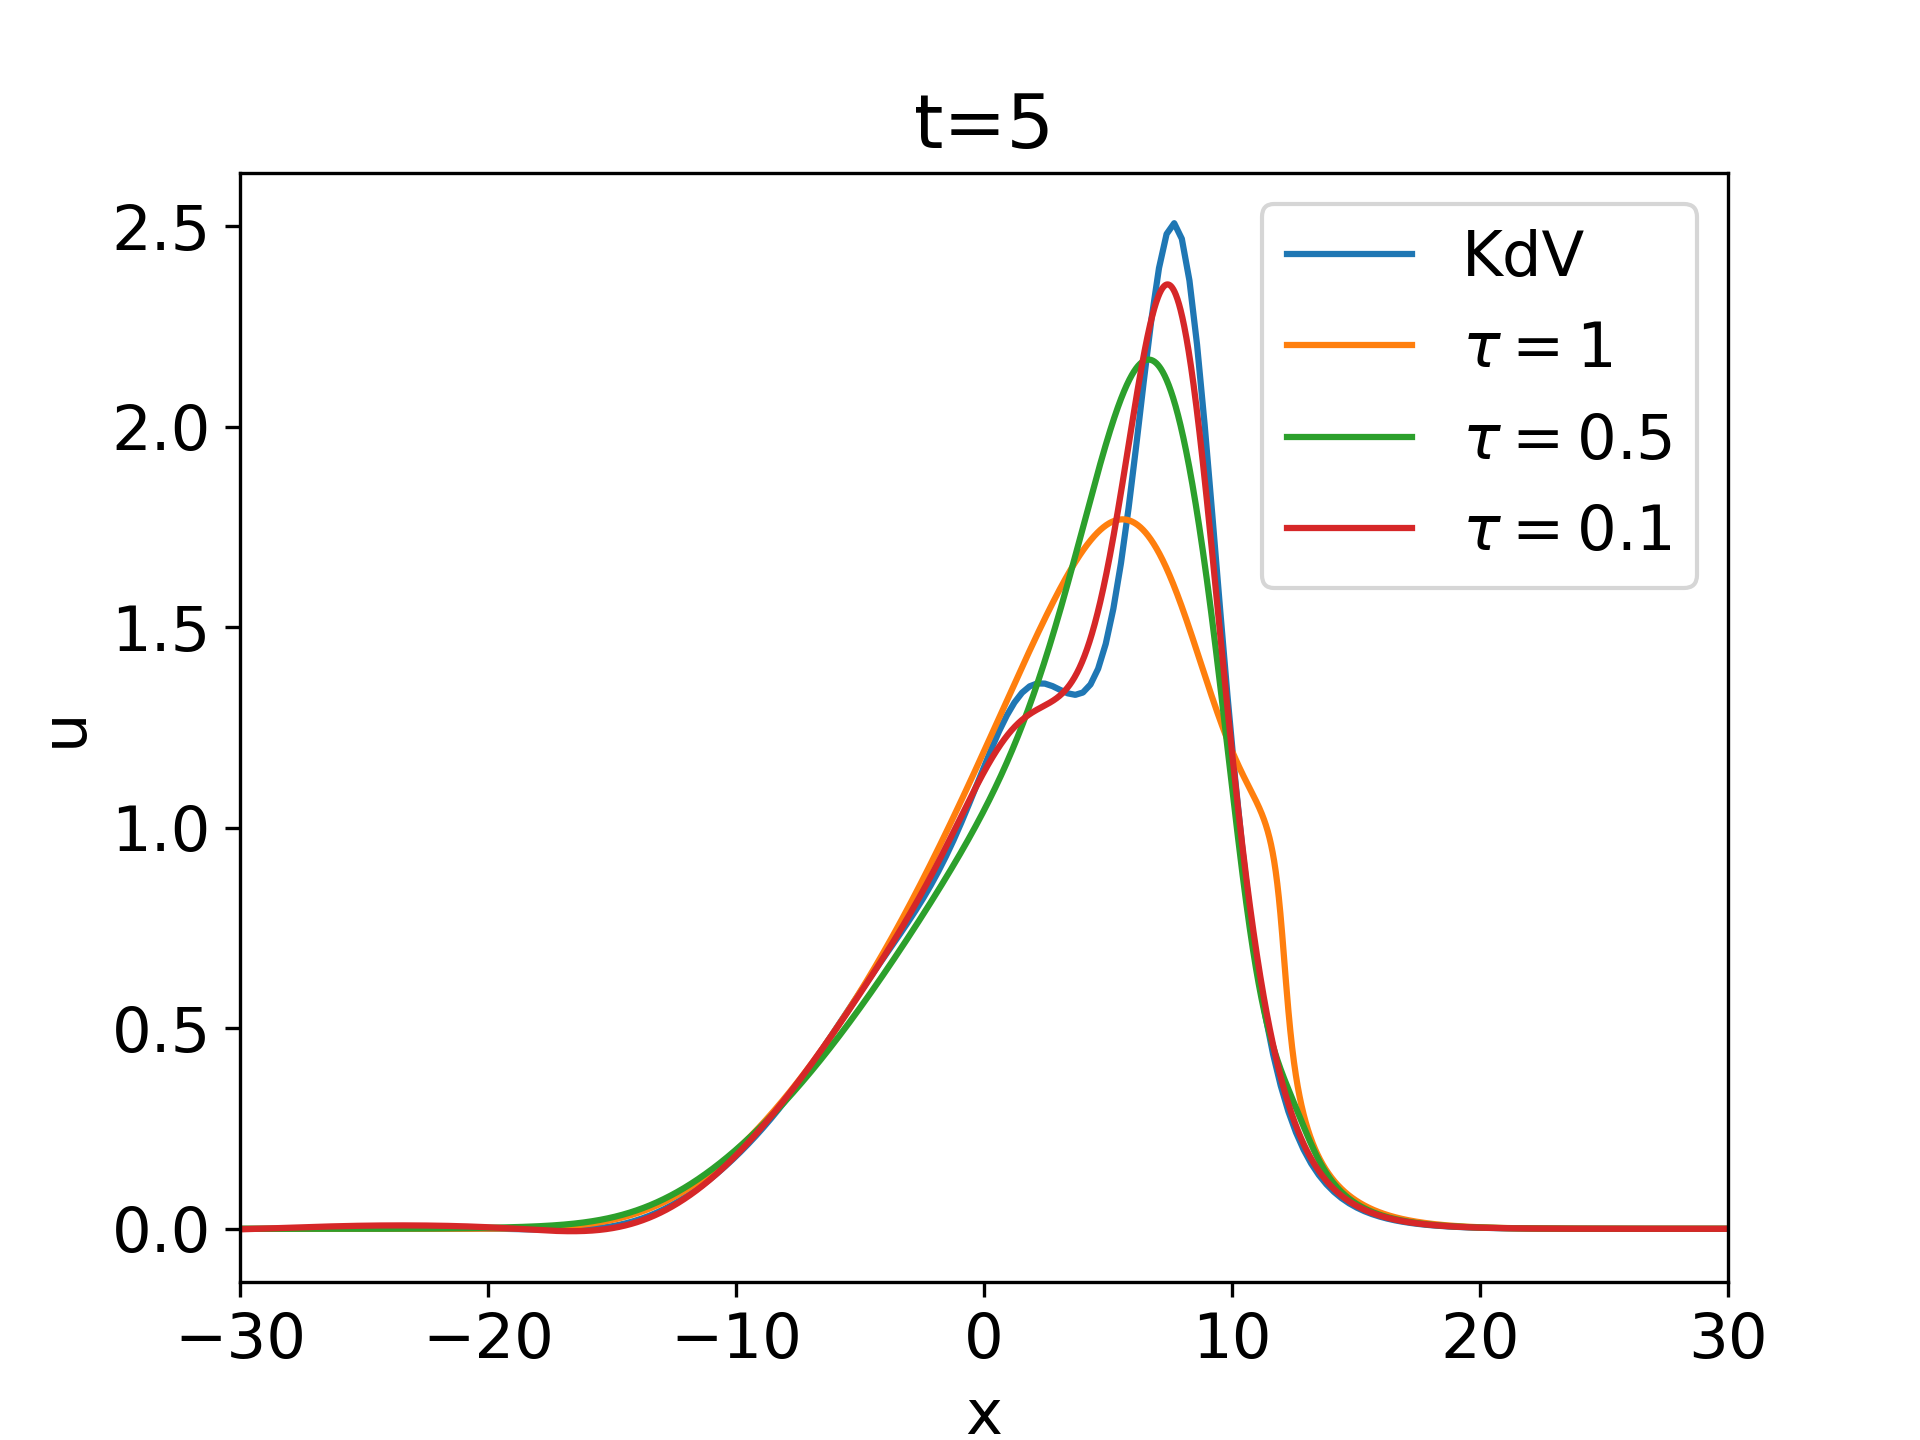
\includegraphics[width=4in]{figures/Convergence.png}
    \caption{Convergence of KdVH solutions to KdV.\label{fig:convergence}}
\end{figure}

In Figure \ref{fig:shocks}, we observe the clear appearance of shocks for $\tau=1$, while
the solution for $\tau=1/10$ is clearly devoid of shocks.

\begin{figure}
\centering
    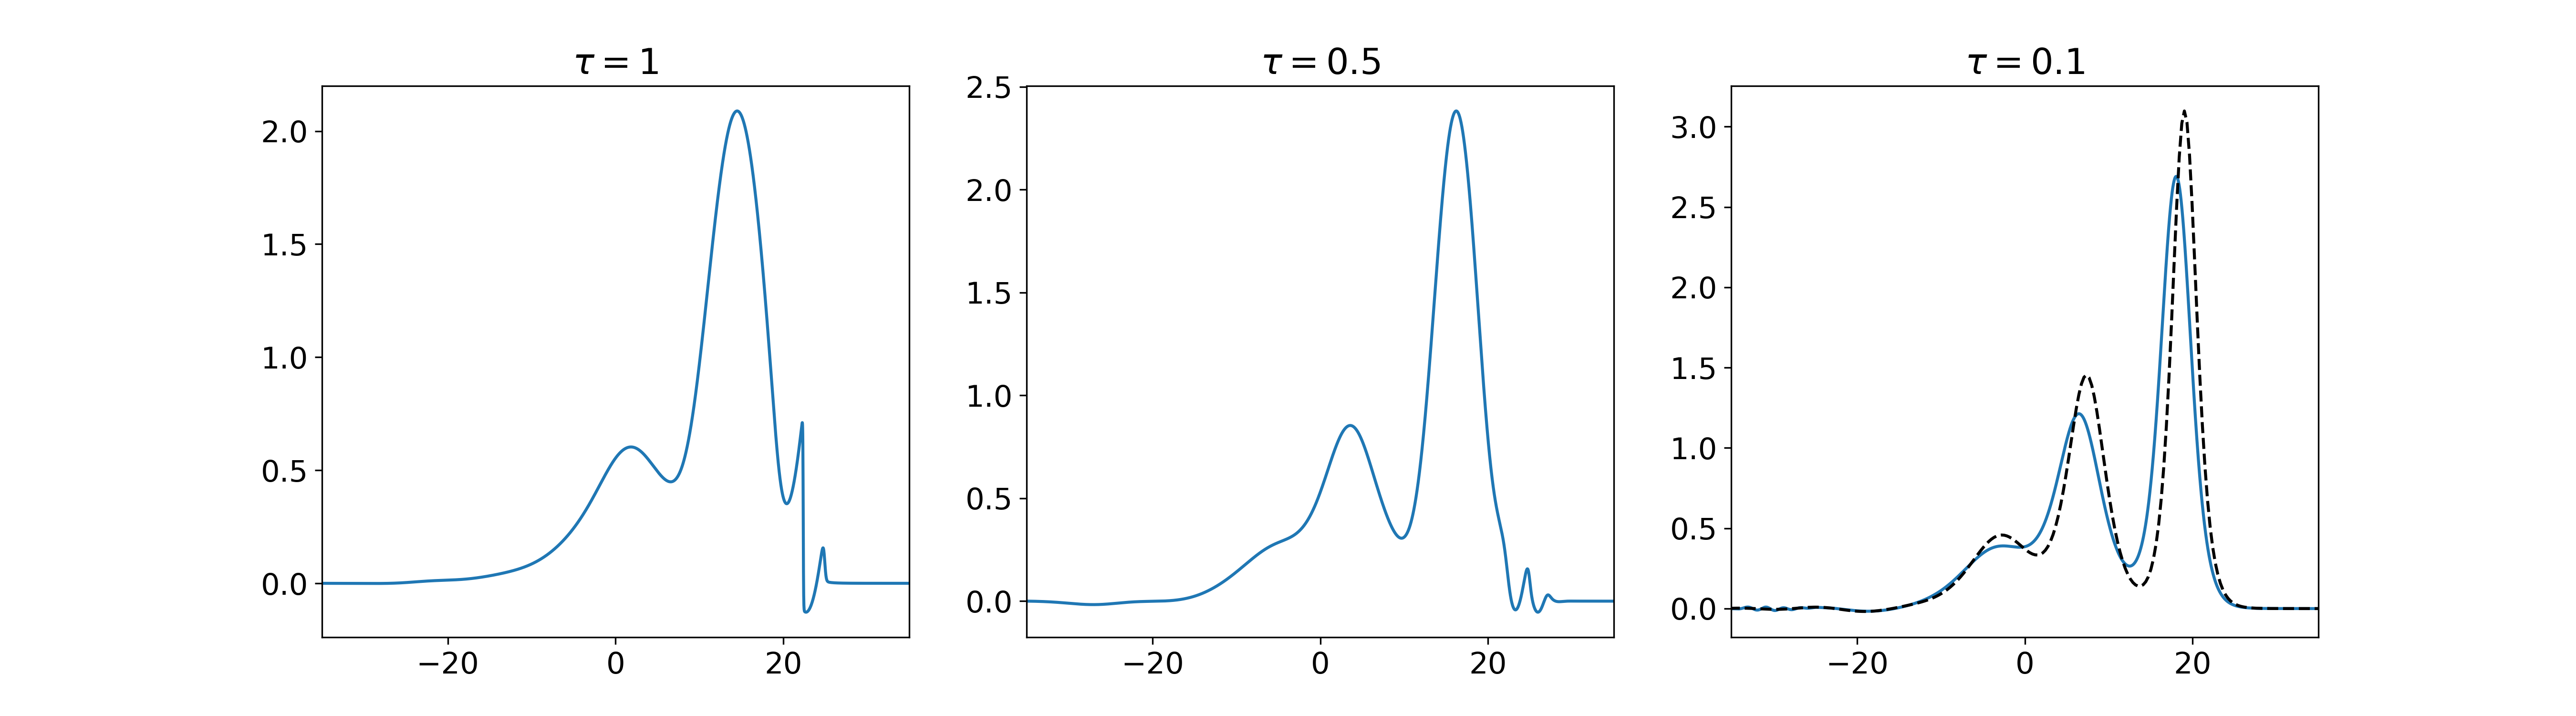
\includegraphics[width=6in]{figures/KdVH_solutions.png}
    \caption{Comparison of solutions at $t=16$.  In the last plot, the KdV solution is included (dashed black line)
    for comparison.\label{fig:shocks}}
\end{figure}


\end{document}

